 %Explicar lo que se hizo

\frame{
\frametitle{Análisis}
\framesubtitle{Instalación API JAAS}
\begin{itemize}
	\item Primer paso.
	\item Más importante para poder realizar todas las configuraciones restantes.
	\item Necesariamente funcional.
\end{itemize}
}

\frame{
\frametitle{Análisis}
\framesubtitle{Integración de LDAP en JBoss usando JAAS}
\begin{itemize}
	\item JBoss con el módulo LoginLdapModule
	\item Configuración módulo para autentificación y autorización mediante JAAS.
\end{itemize}
}

\frame{
\frametitle{Análisis}
\framesubtitle{Integración de JAAS en Tomcat}
\begin{itemize}
	\item Es posible utilizar JAAS como mecanismo de autenticación.
	\item Se pierde flexibilidad una vez autenticado el usuario.
	\item ...aplicación web es otro contexto.
	\item Necesidad de implementar servlets en la implementación de JAAS.
	\item ...con el fin de reforzar control de acceso.
\end{itemize}
}

\frame{
\frametitle{Diseño}

\begin{itemize}
	\item Objetivo principal, acceso a diferentes tipos de sistemas con JAAS (y SSO).
	\item Único Login
	\item ...luego se le asigna rol.
	\item Finalmente el usuario obtiene los permisos necesarios para acceder a aplicaciones
\end{itemize}
}

\frame{
\frametitle{Diseño}
\begin{center}
	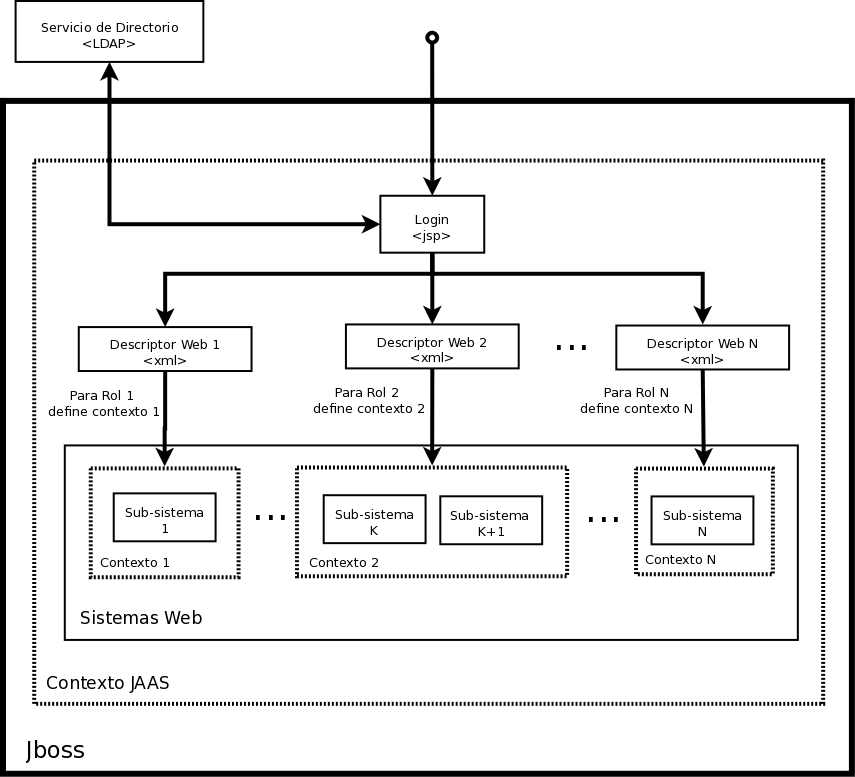
\includegraphics[width=0.7\textwidth]{../reporteTecnico/img/diseno.png}
\end{center}
}

\frame{
\frametitle{Implementación}
\framesubtitle{Instalación de base de datos LDAP}
\begin{itemize}
	\item Bajar e instalar OpenLDAP
	\item Configurar slapd.conf (suffix, rootdn, rootpw, etc)
	\item Tener Usuarios y Grupos que serán usados en JBoss
\end{itemize}
}

\frame{
\frametitle{Implementación}
\framesubtitle{Implementación del SSO en JBoss}
\begin{itemize}
	\item Edición de archivo de configuración en JBoss (server.xml)
\end{itemize}
}

\frame{
\frametitle{Implementación}
\framesubtitle{Integración de LDAP usando JAAS sobre JBoss}
\begin{itemize}
	\item JBoss usa LoginLdapModule para conectarse con LDAP.
	\item Edición de archivo login-config.xml
	\item Conectarse mediante aplicación JAAS (Servlet) 
\end{itemize}
}
